\documentclass{beamer}
\usepackage[utf8]{inputenc}
\usepackage[T1]{fontenc}
\usepackage{xcolor}
\usepackage{comicneue}
\usepackage{graphbox}

\graphicspath{{img/}}

\title{\bf\fontsize{51.59pt}{51.59pt}\selectfont
\includegraphics[align=c,height=1.2em]{cyber.png}party}
\author{Martin Rey}
\date{}

\begin{document}
\begin{frame}
    \titlepage
\end{frame}

\begin{frame}{Verschlüsselung - Was?}
	Verschlüsselung 101: 
	\begin{itemize}
		\item Für alle lesbaren Text so umwandeln, dass er nicht mehr lesbar ist, wenn man keine Berechtigung dazu hat
	\end{itemize}		
\end{frame}

\begin{frame}{Verschlüsselung - Warum?}
    \begin{center}
        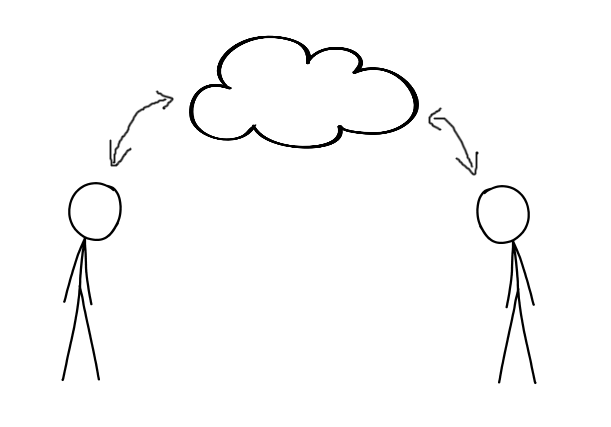
\includegraphics[height=0.6\textheight]{thecloud.png}
    \end{center}
	\begin{itemize}
		\item Man möchte nicht, dass alle wissen, was man macht
		\item Vertrauliche Daten und Personen schützen
	\end{itemize}
\end{frame}

\begin{frame}{Verschlüsselung - Warum?}
	Beispiel 1: Verlust\\
	Ihr verliert euren Notebook im Zug. Durch Verschlüsselung eurer Festplatten verhindert ihr, dass unberechtigte Dritte die Informationen, die auf eurer Festplatte sind, erhalten.
	\\\hspace{1cm}
	
	Beispiel 2: Vertraulichkeit\\
	Ihr wollt miteinander mit der Sicherheit kommunizieren, dass nur berechtigte Personen mitlesen können. Durch verschlüsselte Kommunikationswege macht ihr es schwerer, abgehört zu werden.	
\end{frame}

\begin{frame} {Verschlüsselung - Wie?}
	\begin{itemize}
		\item Open Source: Alle können nachprüfen, wie die Verschlüsselung funktioniert und die Sicherheit liegt nur im Schlüssel.
                \item Aktuelle \& geprüfte Kryptographie: Die Verschlüsselungs-Methode ist bereits länger in Crypto-Kreisen bekannt und es wurden keine Schwächen gefunden.
	\end{itemize}
	
        \pause
	Sinnvoll zu haben:
	\begin{itemize}
            \item Ende-zu-Ende (E2E): Die Verschlüsselung reicht vom Sender bis zum Empfänger.
            \item Glaubhafte Abstreitbarkeit (plausible deniability): Man kann glaubhaft abstreiten, von der Existenz einer Nachricht zu wissen.
	    \item perfect forward secrecy: Auch wenn in Zukunft ein Schlüssel kompromitiert wird, ist alte Kommunikation nicht entschlüsselbar.
	\end{itemize}
\end{frame}

\begin{frame}{Verschlüsselung - Womit? (Messenger)}
    \begin{tabular}{c|ccccccccc}
	& 
\includegraphics[height=1.5em]{whatsapp.png} 
        & 
\includegraphics[height=1.5em]{facebook.jpg}
        & 
\includegraphics[height=1.5em]{threema.png}
        & 
\includegraphics[height=1.5em]{telegram.png}
        & 
\includegraphics[height=1.5em]{signal.png}
        & 
\includegraphics[height=1.5em]{wire.png}
        & 
\includegraphics[height=1.5em]{conversations.png}
        & 
\includegraphics[height=1.5em]{briar.png}
        & 
\includegraphics[height=1.5em]{deltachat.png}
        \\
        {\small Offen} & \textcolor{red}{\bf\Huge-} & \textcolor{red}{\bf\Huge-} & \textcolor{red}{\bf\Huge-} & \textcolor{green}{\bf\Huge+} & \textcolor{green}{\bf\Huge+} & \textcolor{green}{\bf\Huge+} & \textcolor{green}{\bf\Huge+} & \textcolor{green}{\bf\Huge+} & \textcolor{green}{\bf\Huge+} \\
        {\small Crypto} & \textcolor{green}{\bf\Huge+} & \textcolor{red}{\bf\Huge-} & \textcolor{green}{\bf\Huge+} & \textcolor{orange}{\bf\Huge\textasciitilde} & \textcolor{green}{\bf\Huge+} & \textcolor{green}{\bf\Huge+} & \textcolor{green}{\bf\Huge+} & \textcolor{green}{\bf\Huge+} & \textcolor{green}{\bf\Huge+} \\
        {\tiny Infrastruktur} & \textcolor{red}{\bf\Huge-} & \textcolor{red}{\bf\Huge-} & \textcolor{red}{\bf\Huge-} & \textcolor{red}{\bf\Huge-} & \textcolor{orange}{\bf\Huge\textasciitilde} & \textcolor{orange}{\bf\Huge\textasciitilde} & \textcolor{green}{\bf\Huge+} & \textcolor{green}{\bf\Huge+} & \textcolor{green}{\bf\Huge+} \\
        {\small Desktop} & \textcolor{orange}{\bf\Huge\textasciitilde} & \textcolor{green}{\bf\Huge+} & \textcolor{red}{\bf\Huge-} & \textcolor{green}{\bf\Huge+} & \textcolor{orange}{\bf\Huge\textasciitilde} & \textcolor{green}{\bf\Huge+} & \textcolor{green}{\bf\Huge+} & \textcolor{red}{\bf\Huge-} & \textcolor{green}{\bf\Huge+} \\
        {\small "Features"} & \textcolor{green}{\bf\Huge+} & \textcolor{green}{\bf\Huge+} & \textcolor{green}{\bf\Huge+} & \textcolor{green}{\bf\Huge+} & \textcolor{orange}{\bf\Huge\textasciitilde} & \textcolor{green}{\bf\Huge+} & \textcolor{orange}{\bf\Huge\textasciitilde} & \textcolor{red}{\bf\Huge-} & \textcolor{orange}{\bf\Huge\textasciitilde} \\
    \end{tabular}
	
	\hspace{2cm}
	\tiny{weitere Infos auf \url{https://www.securemessagingapps.com/}}
\end{frame}

\begin{frame}{Verschlüsselung - Womit? (Messenger)}
    \begin{itemize}
        \item Signal - \url{https://www.signal.org}
        \item Wire - \url{https://app.wire.com}
        \item Conversiations (Jabber, Android) - \url{https://conversations.im}
        \item Gajim (Jabber, Desktop) - \url{https://gajim.org}
        \item Briar - \url{https://briarproject.org}
        \item Deltachat (E-Mail, Android) - \url{https://delta.chat}
    \end{itemize}
\end{frame}

\begin{frame}{Verschlüsselung - Womit? (E-Mail)}
	Wer benutzt denn noch E-Mails? \\\pause
	\hspace{1cm}
	
	Allgemeines zu E-Mails:
	\begin{itemize}
		\item benutzt Alternativen zu "kostenlosen" E-Mail-Anbietern
		\item gute Beispiele: \url{mailbox.org}, \url{posteo.de}, ...
		\item schlechte Beispiele: \url{gmail.com}, \url{hotmail.com}, ...
	\end{itemize}
	\hspace{1cm}\pause
	
	E-Mail-Verschlüsselung mit PGP kurz gesagt:\\
	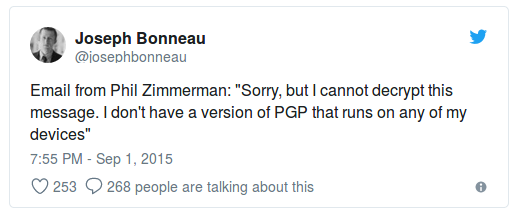
\includegraphics[width=10cm]{phil.png}
\end{frame}

\begin{frame}{Verschlüsselung - Womit? (E-Mail)}
	Autocrypt (\url{https://autocrypt.org/}) ist ein Standard, der Menschen PGP einfacher macht, indem es die Programme "automatisch" verschlüsseln  lässt.\\
	\hspace{1cm}
	
	Welche E-Mail-Programme unterstützen das gerade?
	\begin{itemize}
	\item Deltachat (App)
	\item K9-Mail (App)
	\item Enigmail (Thunderbird Plugin)
	\end{itemize}
	\hspace{1cm}
	
	Und wie benutze ich das nun?
	\begin{itemize}
		\item Lade das Programm herunter und richte dein E-Mail-Konto darin ein. Fertig. Jetzt werden alle E-Mails von und zu Menschen die auch Autocrypt verwenden mit PGP verschlüsselt.
	\end{itemize}
\end{frame}

\begin{frame}{Verschlüsselung (Daten)}
    \center\huge{Daten}               
\end{frame}                           

\begin{frame}{Verschlüsselung - Womit? (Daten)}
	Problem: Je nach Gerät anders :(
    \begin{itemize}
    	\item Aber: Prinzip ist gleich
    	\item Man nutzt ein Programm, dass das Gerät verschlüsselt
    	\item Nur welches Programm?
    \end{itemize}
\end{frame}

\begin{frame}{Verschlüsselung - Womit? (Daten)}
\begin{tabular}{ l | l }
	System & Programm \\\hline
	Windows/Linux & Veracrypt* \\
	Linux & LUKS \\
	Android & Device Encryption \\
	iOS & Device Encryption  \\
\end{tabular}

\hspace{2cm}

*\small{\url{https://www.veracrypt.fr}}
	
\end{frame}

\begin{frame} {Sicherheit - Softwareupdates}
	Euer System wird euch (hoffentlich) sagen, wenn es Updates gibt. Und wenn es sie gibt, installiert sie.
	\\\hspace{1cm}
	
	FAQ:
	\begin{itemize}
		\item Muss ich wirklich alle installieren? \pause
		\\ Ja. \pause
		\\ (oder prüfen, ob im changelog keine security updates sind) \pause
		\item Wie häufig ist es, dass das System nach einem Softwareupdate nicht mehr funktioniert? \pause
		\\ Das ist nicht vorhersagbar, aber selten. \pause
		\item Soll ich es trotzdem installieren/prüfen? \pause
		\\ Ja. \pause
		\item Wieso? \pause
		\\ Wenn dein System kompromittiert ist, bringt sämtliche Verschlüsselung nichts.
	\end{itemize}
\end{frame}

\begin{frame}{Sicherheit - Passwörter}
	\begin{itemize}
		\item Benutzt Passwörter nie, nie mehrmals
                \item Generiert zufällige Passwörter (d.h. verwendet ein Programm)
		\item Benutzt einen Passwortmanager (KeePassXC, password-store, \dots)
	\end{itemize}
\end{frame}

\begin{frame}{Sicherheit - Passwörter}
	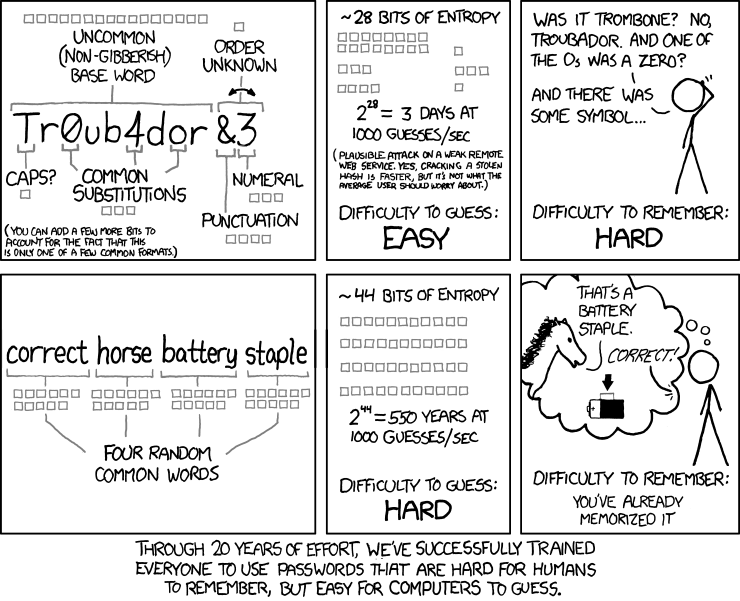
\includegraphics[width=10cm]{password_strength.png}
\end{frame}

\begin{frame}{Sicherheit - Datensparsamkeit}
    \centering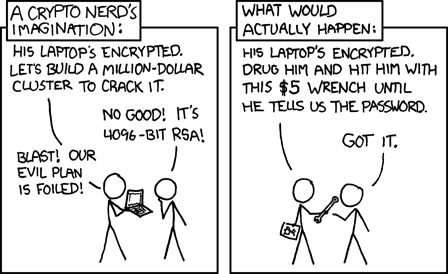
\includegraphics[height=0.7\textheight]{opsec_xkcd.png}	
\end{frame}

\begin{frame}{Anonymität}
	Ist an sich keine Verschlüsselung, sondern wie man sich anonym im Internet verhält.
	\\\hspace{1cm}
	
	Was ist Anonymität?
	\begin{itemize}
		\item Man ist anonym, wenn es nicht identifiziert werden kann
	\end{itemize}
	
	Warum ist das wichtig?
	\begin{itemize}
		\item Es ist sehr einfach verfolgt zu werden, während man im Internet ist. 
	\end{itemize}
\end{frame}

\begin{frame}{Anonymität - 
\includegraphics[align=c,height=1.5em]{tor.jpg}}
	Was ist Tor?
	\begin{itemize}
		\item Kurz für "The Onion Router"
		\item Tor-Browser hilft, anonym zu sein
		\item (außerdem gibt es Websiten, die man nur mit diesem Browser erreichen kann)
		\item Kann man herunterladen auf \url{https://www.torproject.org/} und einfach starten
	\end{itemize}
	\hspace{1cm}
	
	Wie funktioniert es?
\end{frame}

\begin{frame}{Anonymität - 
\includegraphics[align=c,height=1.5em]{tor.jpg}}
    \centering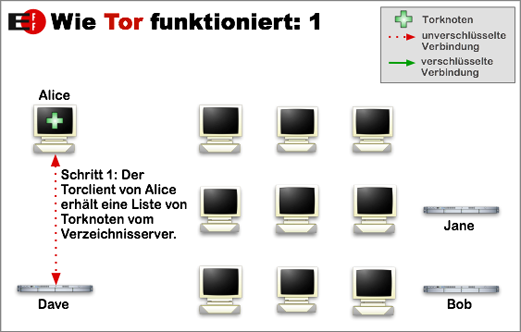
\includegraphics[height=0.7\textheight]{tor1.png}
\end{frame}

\begin{frame}{Anonymität - 
\includegraphics[align=c,height=1.5em]{tor.jpg}}
    \centering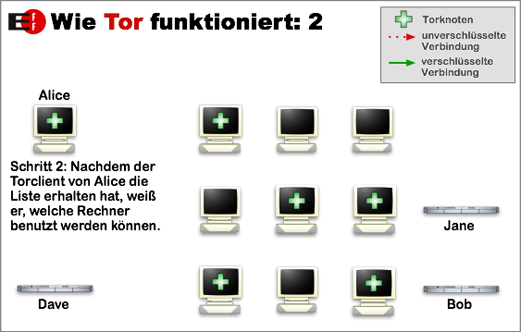
\includegraphics[height=0.7\textheight]{tor2.png}
\end{frame}

\begin{frame}{Anonymität - 
\includegraphics[align=c,height=1.5em]{tor.jpg}}
    \centering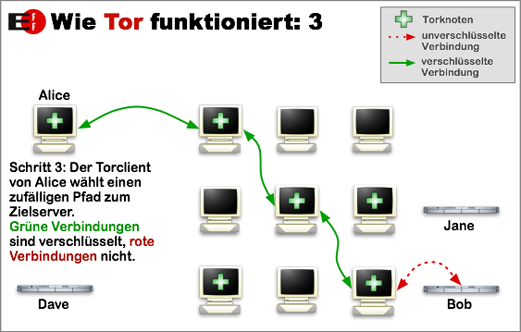
\includegraphics[height=0.7\textheight]{tor3.png}
\end{frame}

\begin{frame}{Anonymität - 
\includegraphics[align=c,height=1.5em]{tor.jpg}}
    \centering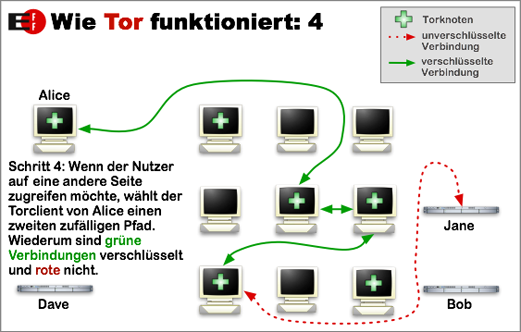
\includegraphics[height=0.7\textheight]{tor4.png}
\end{frame}

\begin{frame}{Anonymität - 
\includegraphics[align=c,height=2.3em]{tails.png}}
	Was ist das?
	\begin{itemize}
		\item TAILS ist ein Betriebssystem, das zum Ziel hat, anonymes Verhalten im Internet sicher und einfach zu machen.
		\item Tor und andere Werkzeuge vorinstalliert
                \item Speichert keinerlei Daten!
	\end{itemize}
\end{frame}

\begin{frame}{Namensnennung}
	\begin{itemize}
        \item xkcd Webcomic - \url{https://www.xkcd.com}
        \item "CYBER" Bild: CC-BY-NC fnordeingang e.V. \url{https://fnordeingang.de}
    \end{itemize}
\end{frame}

\end{document}
